\chapter{Introduction}

%citazione introduttiva
\epigraph{\textit{How do you know if what you believe is really true?}}{}


This chapter introduces the background of this work identifying its relevance, originality and the placement within the existing literature.\par

The background of this work is engineering. Engineering is composed of models based on math (approximations) that describe a physical phenomenon. The electricity current passing through a wire, the lift force of the air which supports the weight of an aircraft, the exchange of heat in an air conditioning system are physical phenomenon described by engineering models. On-field experiments and observation lead to the definition of the models, i.e. the mathematical relationships between the entities involved in the phenomenon.

\section{Taxonomy} \label{secSupplyChainTaxonomy}

Logistics research is the research domain of this work, which is borderline between engineering and economics. The world \textit{taxonomy} comes from the ancient Greek \textgreek{τάξις} (order) and \textgreek{νόμος} (law). A taxonomy is used to classify the disciplines of a research domain systematically. Figure \ref{fig_operationsResearch} proposes a taxonomy of the logistics research domain. Table \ref{tab_glossaryIntroduction} introduces the glossary with the keywords of this taxonomy.

% INSERT fig_operationsResearch
\begin{figure}[hbt!]
\centering
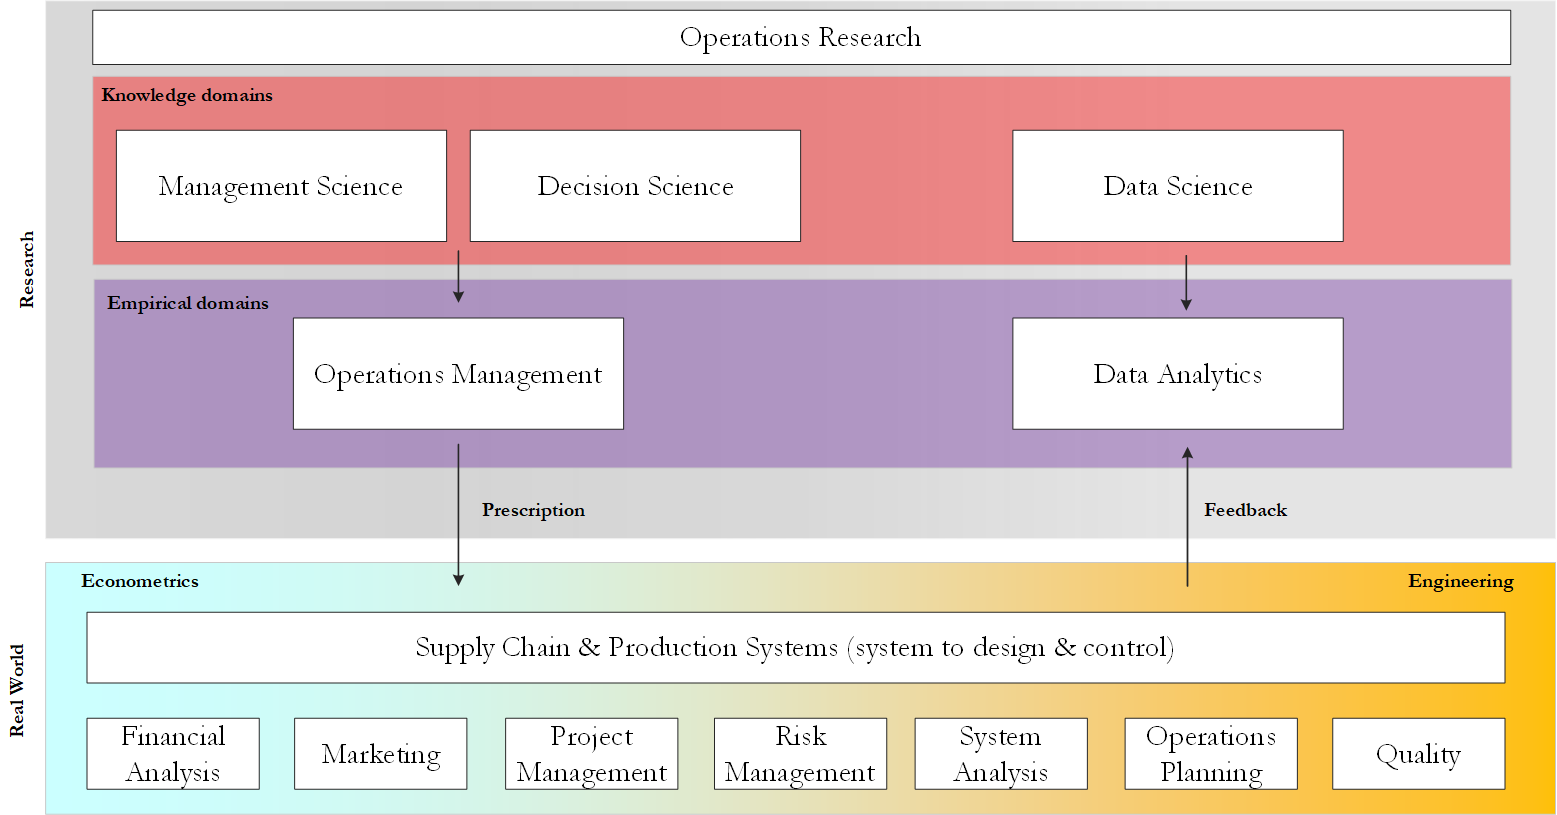
\includegraphics[width=1\textwidth]{SectionIntroduction/introduction_figures/fig_operationsResearch.png}
\captionsetup{type=figure}
\caption{Taxonomy of operations research}
\label{fig_operationsResearch}
\end{figure}


% Please add the following required packages to your document preamble:
% \usepackage{graphicx}
\begin{table}[]
\caption{Glossary of opertions research.}
\label{tab_glossaryIntroduction}
\resizebox{\textwidth}{!}{%
\begin{tabular}{ll}
\hline
Keyword                            & Description                                                                                                                                             \\ \hline
Research domain                    & contributions of academic research on a specific topic.                                                                                                 \\
Real World                         & a physical system.                                                                                                                                      \\
Operations Research                & a research discipline studying the operations (e.g., storage, distribution and production) in the supply chain.                                         \\
Management Science                 & a research discipline studying the relationship between people and resources in an operational context.                                                 \\
Decision Science                   & a research discipline studying the outcome of people’s decisions or expert systems in an operational context.                                           \\
Data Science                       & a research discipline   studying the information content of data.                                                                                       \\
Operations Management              & the outcome of   management and decision science, i.e. a set of models to design and control a   supply chain.                                          \\
Data Analytics                     & a set of models to understand and analyse the information content of a dataset.                                                                         \\
Supply Chain \& Production systems & the set of physical and virtual entities implementing technologies for the realisation, storage and transportation of goods.                            \\
Financial Analysis                 & application of a set of methods to identify the financial position of a physical (e.g., an asset) or virtual (e.g. a stock) entity in the supply chain. \\
Marketing                          & application of a set of methods to connect the demand and offer of a product/service.                                                                   \\
Project Management                 & application of a set of methods to manage resource and time for the realisation of a project.                                                           \\
Risk Management                    & application of a set of methods to manage and control the risk connected to the entities of the supply chain.                                           \\
System Analysis                    & application of a set of methods to manage and control the behaviour of a set of entities in the supply chain.                                           \\
Operations Planning                & application of a set of methods to manage resource and time for the realisation of the product/service.                                                 \\
Quality                            & application of a set of methods   to keep the operations under statistical control.                                                                     \\ \hline
\end{tabular}%
}
\end{table}

This work considers the relationship between decision science and data science proposing a new role of data analytics as a prescriptive tool (together with operations management). The \textit{System Analysis} is the field of application of this work in the supply chain. The following paragraphs introduce the topology for decision \ref{secDecScienceTopology} and data science \ref{secDataScienceTopology}.

\section{Decision Science Topology} \label{secDecScienceTopology}
The word \textit{topology} comes from the ancient Greek \textgreek{τóπος} and \textgreek{λóγοσ}, literally place and study. Differently from taxonomy, the topology studies the “space” of a discipline. In this case, we want to explore which variables influence the nature of the tools used in decision and data science.\par

To define the object of study of this work, we consider the literature ~\cite{Stecca2019} classifying a decision-making process according to:

\begin{itemize}
    \item the number of decision-makers;
    \item their knowledge about the information relevant to the decision. 
\end{itemize}

Usually, a decision-maker (DM) makes a decision (i.e., setting the value of decision variables) based on the knowledge of some information (i.e., decision parameters).\par

A decision process can have single or multiple DMs. We define, accordingly, concentrated and distributed decision making. The information for the decision-making process can be centralised within a single entity/actor or decentralised and owned by several sources. Depending on the topology of information and decision-makers, there are different tools to support the decision process. Figure \ref{fig_decisionsParMak} illustrates this decision topology with classic decision science tools. We analyse four different cases (CC, CD, DC and DD).

% INSERT fig_decisionsParMak
\begin{figure}[hbt!]
\centering
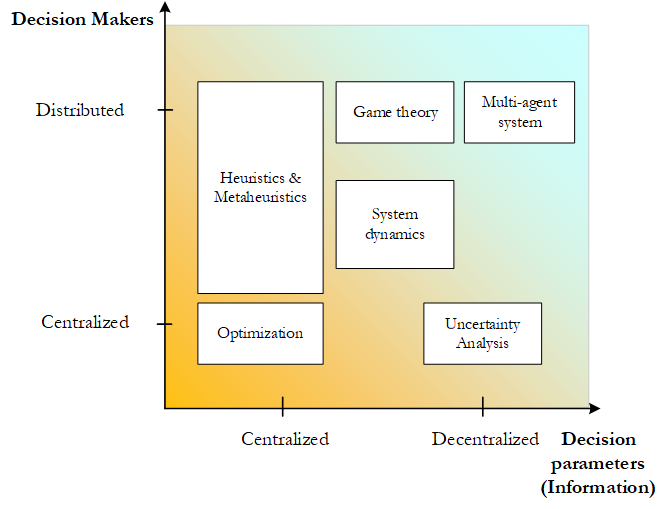
\includegraphics[width=1\textwidth]{SectionIntroduction/introduction_figures/fig_decisionsParMak.png}
\captionsetup{type=figure}
\caption{The Taxonomy of deision support methods.}
\label{fig_decisionsParMak}
\end{figure}

\subsection{Centralised information with centralised decision-makers (CC)}
When a single DM knows all the decision parameters, the optimisation (e.g. integer linear programming, nonlinear programming, robust optimisation) is the most used decision support tool. When the complexity of an instance arises, the optimisation runtime increases exponentially. Under these conditions, suboptimal heuristics or metaheuristics are good alternatives to get proper results within a brief time. A vast number of operational decisions belong to this group since a single person (i.e. the manager) has the responsibility for the decision and the ownership of the information. Some examples are:

\begin{itemize}
    \item the definition of the storage assignment in an industrial storage system;
    \item the job scheduling on a production machine;
    \item the loading sequence of the containers on a vessel;
    \item the definition of the route for a fleet of trucks.

\end{itemize}

An intermediate decision support tool between CC and DC is the “system dynamics”, which defines connection and cause-effect relationships between the decision variables (i.e. the entity of a system) and the DMs. The relationships are usually nonlinear, and the system dynamic evolves at different time steps. The discrete event simulation (DES) is an implementation of system dynamics which evaluates the states of a system at discrete time lags.

\subsection{Centralised information with distributed decision-makers (CD)}
When the output of a single DM depends on the information owned by other DMs, it is necessary to identify different decision scenarios guessing the behaviour of the other actors. Usually, two tools go in this direction:

\begin{itemize}
    \item game theory;
    \item specific heuristics or metaheuristics algorithms.
\end{itemize}

The game theory assesses the probability of the outcomes of a decision process evaluating all the alternatives in a tree structure. Game theory is mostly used to evaluate the payback of many actors cooperating or not cooperating in a supply chain. All the possibilities of cooperation or not cooperation are evaluated, finding the payback for each actor. Different strategies exist to identify the strategy which provides a higher benefit to a single actor or the entire system.\par

Heuristics and metaheuristics result suitable to provide sub-optimal solutions since they can e tailored to a specific instance of the problem.\par

The definition of the route of a truck is an example of this problem: the planner has all the information, but some decisions (e.g. route replanning) may happen due to exogenous facts as disruptions. 

\subsection{Decentralised information with distributed decision-makers (DD)}

When the information and the ownership of the decision are decentralised, the outcome of the decision process depends on several independent decisions for each actor of the system. An important support tool is the agent-based modelling where each actor (i.e. an agent) has its own set of (partial) information to base its decision. Multi-agent simulation is similar to discrete event simulation. However, each actor implements its specific heuristics to make decisions based on the current state of the system from his point of view (i.e. based on its information set). \par

The participation of a company to a tender is an example of DD; each company makes an offer based on its information. The outcome of the process depends on all the offers from all the companies participating in the tender.

\subsection{Decentralised information with centralised decision-makers (DC)}
When a single DM has the ownership of the decision but not all the information needed, the analysis of the uncertainty is a good choice to deal with the decision process. There are statistical models and methods to evaluate the risk behind a decision (e.g. Montecarlo simulation), and it is possible to infer information finding integrity rules among data. \par

Any CC case with incomplete knowledge on the decision parameters is a DC decision process. The incompleteness can be approached using statistical approaches as Montecarlo simulation or Markov chain to identify confidence intervals on a target variable. It is the case of cost-benefit analysis, where some cost distributions are skewed or hard to estimate.

This book focuses on centralised decision making in the supply chain, i.e. CC and DC cases.


\section{Data Science Topology} \label{secDataScienceTopology}

The previous paragraph introduces a topology of the most used decision support methods without paying attention to the type of data they need. First of all, it is necessary to classify the input data depending on their structure:

\begin{itemize}
    \item structured data. These data usually are from a relational database (e.g., SQL-based) designed using an entity-relationship (ER) model;
    \item Semi-structured data. These data come with a precise but non-relational structure (e.g. CSV, NO-SQL, XML and JSON\footnote{JavaScript Object Notation.} data);
    \item unstructured data. These data have no structure (e.g. text, pictures).
\end{itemize}

In the majority of cases, the literature on logistics and operations works with structured data. Usually, scholars and researchers first approach the methodology to solve a problem and then look for data to validate the approach (model-driven approach). These data are rarely available, and a considerable part of the literature on decision sciences relies on theoretical models validated by randomly generated instances. This research approach supports the development of robust and efficient algorithms, but it does not address real problems. Besides, there is a risk that the problem identified by the researchers does not exist in practice.\par

In this work, we use a different perspective, by introducing the data-driven approach, that is based on the classification in ~\cite{Irv2010} (see Figure \ref{fig_methods}). Data-driven means “let data speak for itself”. The major effort is on understanding the meaning of data and developing a decision support method only after translating data into information.

% INSERT fig_methods
\begin{figure}[hbt!]
\centering
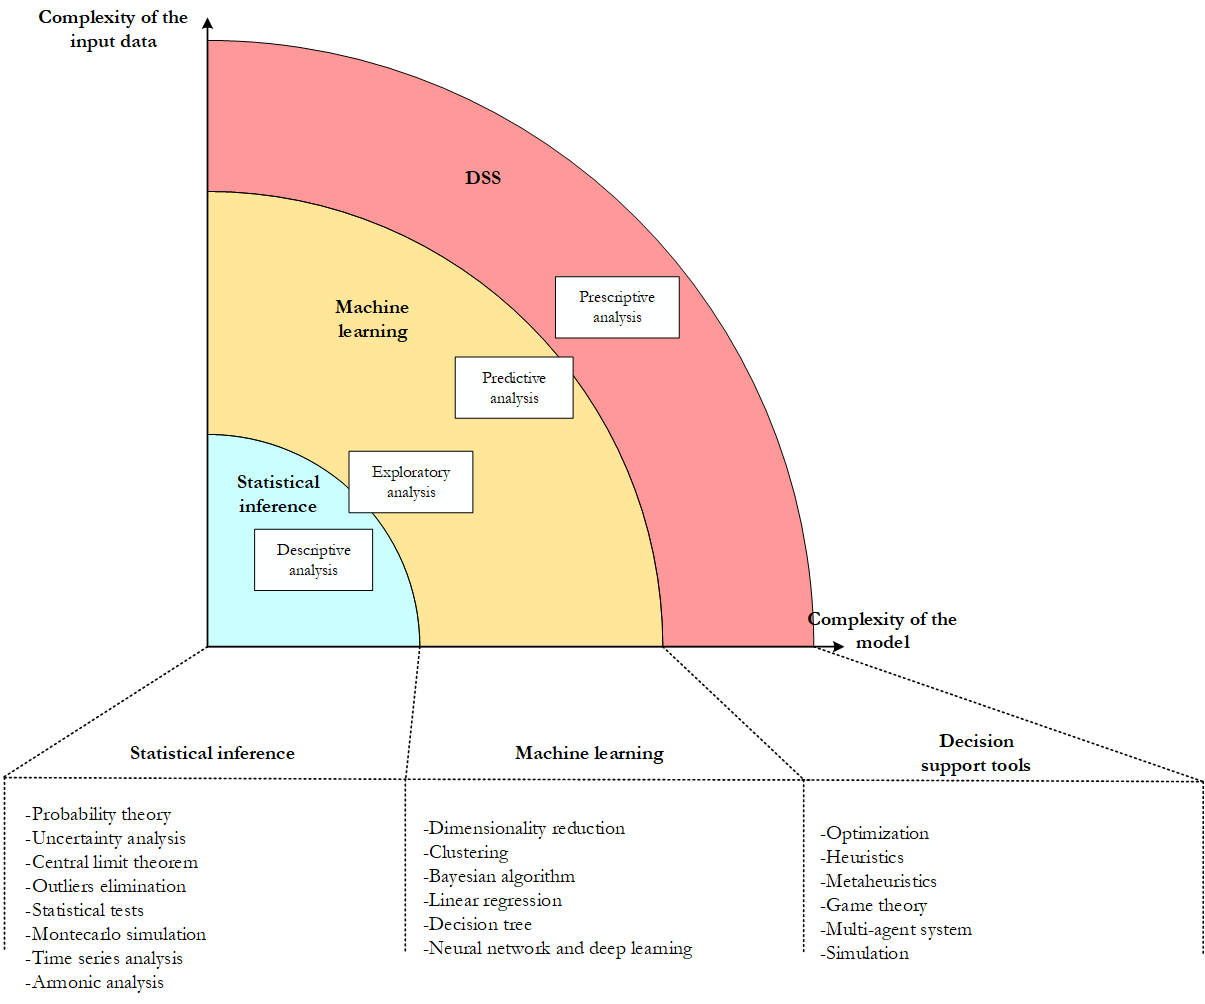
\includegraphics[width=1\textwidth]{SectionIntroduction/introduction_figures/fig_methods.png}
\captionsetup{type=figure}
\caption{The relationship between data and analyticsl methods.}
\label{fig_methods}
\end{figure}

During the last decade, scholars pay attention to data science because of the advent of big data. Big data is the collection, storage and manipulation of data that are \cite{Kitchin2014}:

\begin{itemize}
    \item Huge in storage volume;
    \item High in velocity (e.g., real time);
    \item Diverse in variety (e.g., structured/semi-structured/unstructured);
    \item Exhaustive in scope (i.e., getting the information of a whole population)
    \item Fine-grained in resolution and uniquely indexical;
    \item Relational (i.e., with attributes lining different datasets);
    \item Flexible (i.e., can easily add new attributes);
    \item Scalable (i.e., can easily add new records).

\end{itemize}

Under the perspective of big data, data science opens a new horizon for science. Traditionally, statistical techniques are used to extract knowledge from scarce and static data with weak relations between datasets. This analysis served to answer specific questions (generated under restrictive assumptions) by a researcher with a clear research question in mind ~\cite{Miller2010}. This perspective is changed by big data whose characteristics provides a level of information to explore phenomena without a specific question in mind. Data science introduces a new research paradigm (see Table \ref{tab_paradigms}): Exploratory Science ~\cite{Hey2009}. 


% INSERT tab_paradigms
\begin{figure}[hbt!]
\centering
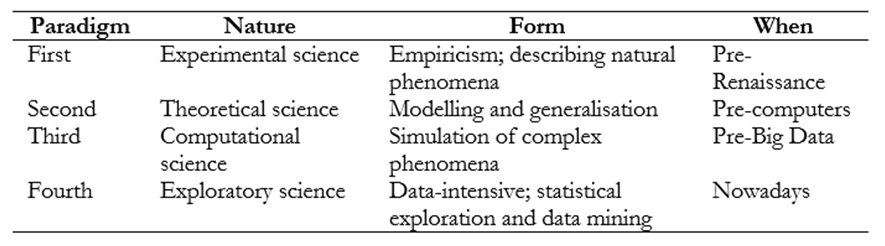
\includegraphics[width=1\textwidth]{SectionIntroduction/introduction_figures/tab_paradigms.png}
\captionsetup{type=table}
\caption{The four research paradigms and their features.}
\label{tab_paradigms}
\end{figure}

The following chapters of this book aim at evaluating when data-driven methods are suitable to address strategic decisions in the field of logistics and operations.

\subsection{Fundamental concepts of data science}
We start, first, from the fundamental theoretical concepts of data science ~\cite{Provost2013}. 

\begin{enumerate}
    \item Extracting useful knowledge from data to solve business problems can be treated systematically by following a process with reasonably well-defined stages.
    \item Evaluating data-science results requires careful consideration of the context in which they will be used.
    \item The relationship between the business problem and the analytics solution often can be decomposed into tractable subproblems via the framework of analysing expected value.
    \item Information technology can be used to find informative data items from within a large body of data.
    \item Entities that are similar with respect to known features or attributes are similar with respect to unknown features or attributes.
    \item If you look too hard at a set of data, you will find something—but it might not generalise beyond the data you’re observing.
   \item To draw causal conclusions, one must pay very close attention to the presence of confounding factors, possibly unseen ones.

\end{enumerate}

The following paragraph comes from the (2) and (3) proposing a framework for logistic and operational data. The other points are implemented in the following sections of this work that are dedicated to storage systems, distribution networks and production plants.

\section{History of Operations Research}
Section \ref{secSupplyChainTaxonomy} introduced the research field of this work, while sections \ref{secDecScienceTopology} and \ref{secDataScienceTopology} review the organisation of the decision support tools belonging to the fields of Decision Science and Data Science. The careful readers already will have noticed some overlaps between these two disciplines. Nevertheless, to understand these overlaps and to point out the direction of this work, it is necessary to introduce some history of the operations research (that, in our taxonomy, embeds both Decision and Data Science). \par

Logistics research was born in 1910 with the term “scientific management”, and it is possible to identify eight different periods where technologies, decision making and quantitative methods embed different roles within the same research domain ~\cite{Mortenson2015}:

\begin{enumerate}
    \item Scientific Management (1910-1945)
    \item Scientific Method (1945-1965)
    \item Management Information System (1965-1970)
    \item Decision Support System (1970-1990)
    \item Business Intelligence (1990-2005)
    \item Analytics (2005-2015)
    \item Artificial Intelligence (2015-today)
    \item Non-Human Intelligence (future)

\end{enumerate}

The scientific management of the work (1) starts together with the first assembly line to produce the Ford Model T. For the first time there is a scientific organisation of the work and the time and motion analysis are used to measure and control the productivity of the line. It is the beginning of the application of scientific tools to operations, the era of logistics research began.\par

In the second period (2), after World War II, the von Neumann architecture defines how to connect the component of a computer. This architecture changed the world, implementing the separation of the processor and the storage unit of a computer. This architecture is still used today in almost all IT applications, and it opened for the implementation of many decision support tools we still use nowadays.\par

The third period (3) has seen the development of microchips, which make affordable for companies to build information technology (IT) systems. Companies started to collect and store data on their operations into their system.\par

In the fourth period (4), these data are used to improve the decision process through: 

\begin{itemize}
    \item decision support systems (DSS), providing the decision-makers with a suggestion to their problem;
    \item expert system (ES), guiding the DM step by step to get a suggestion to his/her problem.

\end{itemize}

During the period of business intelligence (5), it becomes obvious that there is a value behind the data collected by the IT systems. In addition to companies, the world wide web started providing tons of data and information to a broad public.\par

The period of analytics (6) saw the realisation of the deductive process where information is obtained from tons of data and used to understand and improve the operations. Mathematics is used for understanding the data, but human intuition is still necessary to choose and implement the right decision. According to ~\cite{Mortenson2015}, period (6) is the current one. Nevertheless, the technological developments of the last few years move us to add two additional periods.\par

The period of artificial intelligence (7) starts in 2015 when a team of data scientist from Google develops a neural network able to play the game of Go better than the world champion of this game ~\cite{Silver2016}. It is the advent of artificial intelligence. IT systems have already overcome the speed of the human brain (during period 6), but now they are also able to think and react similarly to a real human brain. The following step is theoretical, but natural (8): when the artificial systems will be able to program themselves, they will be able to understand a problem autonomously and to get a solution faster and better than a real human brain. However, for the sake of our knowledge, this step in the history of IT is yet to come.\par

This work focuses on step (6) in the field of logistics and operations. We want to approach analytics to deeper investigate how human intuition and the value of logistics information match for proper management of a supply chain ~\cite{Arvan2019}.\par

Accordingly to the periods defined above, step (6) should already be out-to-date. Nevertheless, the literature (see chapter 2) shows that few papers study analytics from a research point of view and their application in the logistics practice is still rare. The majority of supply chain systems stopped at the stage (4) where complex ES and DSS are seen as the final weapon against the inefficiencies of the supply chain.\par

Big companies use analytics to profile customers, price products and make financial analysis (the green shade in Figure 1). Nevertheless, they rarely studied analytics for engineering applications whose potential is even higher due to big data available from production, tracking and other activities in a supply chain. 

\section{A change in the perspective}

Figure \ref{fig_operationsResearch} illustrates the topology of logistics research and the traditional role of decision science and data science. Here we want to investigate their role from a control perspective. Traditionally, decision science is used to model the system to control (e.g. a supply chain or a plant), and data science is used to get relevant data and keep the variables of the system under control. Figure \ref{fig_controlDataDriven} illustrates the differences between a data-driven and a model-driven approach ~\cite{Hedgebeth2007}, which will now be investigated, from a system control perspective. It is important to remark that a model is never the reality, but a useful approximation used to get information on it ~\cite{Hazen2014}.

% INSERT fig_controlDataDriven
\begin{figure}[hbt!]
\centering
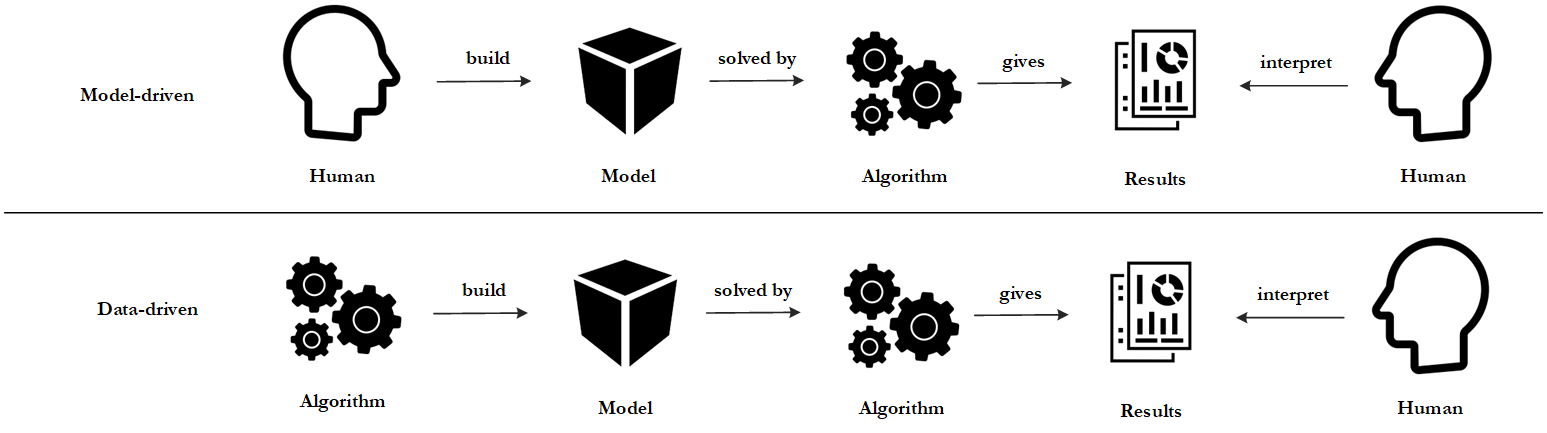
\includegraphics[width=1\textwidth]{SectionIntroduction/introduction_figures/fig_controlDataDriven.png}
\captionsetup{type=figure}
\caption{Model-driven vs. data-driven learning process.}
\label{fig_controlDataDriven}
\end{figure}

The traditional model-driven approach can be seen as a system to control through a feedback loop:

\begin{enumerate}
    \item the real system is modelled through decision science, defining decision variables based on the human understanding of the system. 
    \item the historical data of the system is the input parameter of the model.
    \item the output of the model is analysed and used again to control the system.

\end{enumerate}

Here we have a traditional model-driven approach (see Figure \ref{fig_controlAsIs}) where the “system model” is an ES or a DSS.

% INSERT fig_controlAsIs
\begin{figure}[hbt!]
\centering
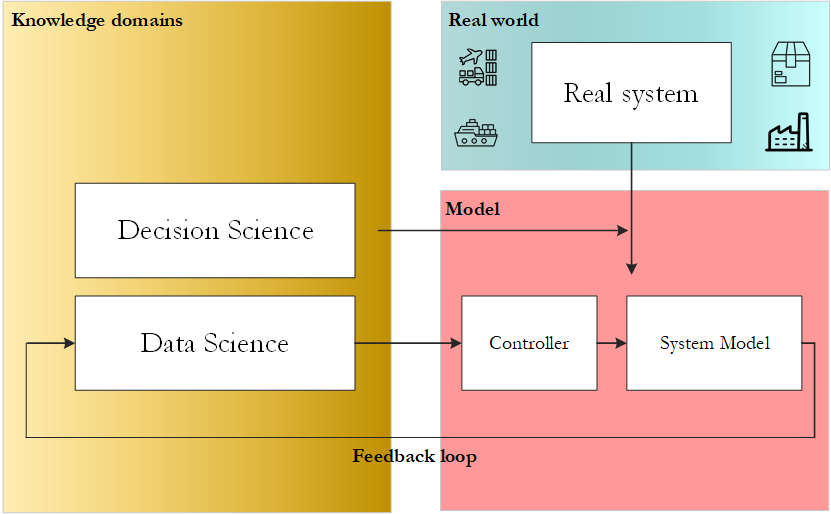
\includegraphics[width=1\textwidth]{SectionIntroduction/introduction_figures/fig_controlAsIs.png}
\captionsetup{type=figure}
\caption{Traditional model-driven approach, based on feedback control.}
\label{fig_controlAsIs}
\end{figure}

In this work, we introduce a different approach (see Figure \ref{fig_controlToBe}). Data science is not only the base for the control of the system but also the design of the model. Figure \ref{fig_controlDataDriven} already illustrated the different between model-driven to data-driven perspectives.

% INSERT fig_controlToBe
\begin{figure}[hbt!]
\centering
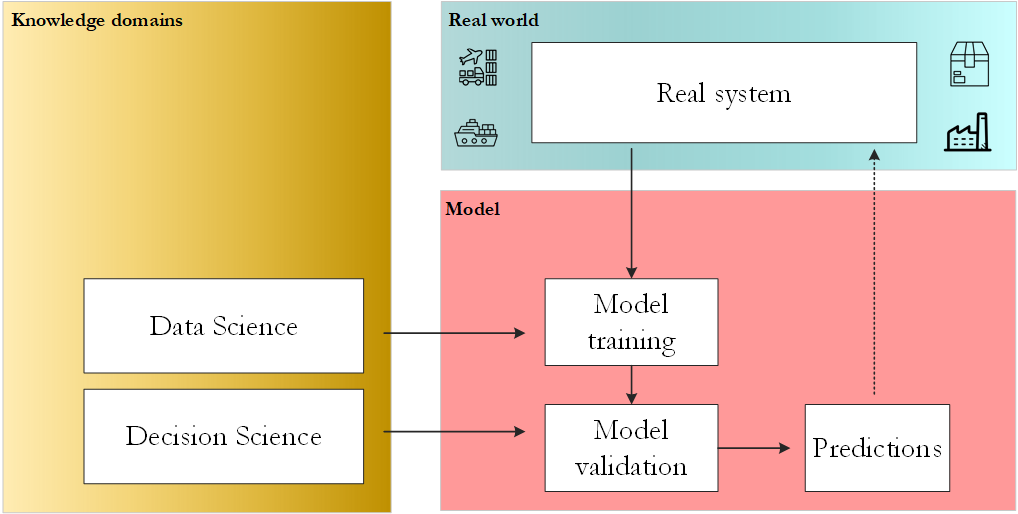
\includegraphics[width=1\textwidth]{SectionIntroduction/introduction_figures/fig_controlToBe.png}
\captionsetup{type=figure}
\caption{Novel data-driven approach, based on predictions.}
\label{fig_controlToBe}
\end{figure}

By using this approach, data science is used to train a model which is based on the real behaviour of the system and not on apriori human intuition. The outcome of the model which highlight patterns, correlation and relationships among data are discussed and interpreted by human and used as input for decision-making. The model is, then, used to predict the behaviour of the system in the future. The model is trained and updated each time new historical data from the real system are available, making the data-driven approach flexible and up-to-date. We can think of this fact as the change from a world where there was the need to design from scratch to a world where Is it necessary to understand, control and improve the extant processes. This is the reason why the following sections of this book analyse the control of a logistic system first.\par

This approach does not question the relevance of decision science, but it considers a new relationship between data science and decision science. We can exemplify this new relationship thinking of the design of a DSS. We identify the four fundamental stages in the design of a DSS from a data-driven perspective (whose implementation will be the object of Parts III, IV and V of this book):

\begin{enumerate}
    \item diagnosis of the real system (business-as-usual);
    \item training of the model;
    \item validation of the model;
    \item deployment of the DSS.

\end{enumerate}

The diagnosing of the business-as-usual scenario (1) is the phase where the DM assesses the problem, its environment, its criticalities, identify the managerial question to answer and the KPIs to measure the goodness of possible answers. In this phase, the DM takes a “snapshot” of the real system using statistical inference and data visualisation to:

\begin{itemize}
    \item understand the business-as-usual process;
    \item identify the level of information at his/her disposal.

\end{itemize}

The training of the model (2) is the phase where the decision variables are identified and the model to predict their value is built (based on data science methods). The model is trained upon the available data from the real world. Differently from the model-driven approach, we do not assume any relationship between the input variables. In some case, assumptions are made on the value of each column to clean the data but, in general, we are interested in augmenting the knowledge we have on the data by only observing the data. For this reason, other assumptions are discouraged at this stage. The model will highlight the relationships between the input data and the decision variables.\par

Human intuition is then required to understand the output of the model and the link between the input data that is the validation of the model (3). Decision science methods can be implemented at this stage when the scenario is complex, and it requires additional information to be useful for the DM (e.g. it is necessary to merge the result of two models trained on different decision variables).\par

When the output of the model is considered confident enough for the DM (and from a statistical point of view), the model can be deployed into a DSS (e.g., a software) able to get input, train the model and present the output aiding the DM in his/her work.\par

This work proposes a novel approach where data-driven models are used together with the traditional scholars’ model-driven approach. In other words, instead of modelling a logistic/operations process based on human understanding, the modelling phase is based on the data available from the measurement of that process.\par

A human effort is required in the organisation of the measurement data and the understanding of the outcome of the model. In other words, we switch from the control of a logistic/operation process to the prediction of the outcome of that process. In this work, we use the terms “data-driven”, “logistics 4.0”, “smart logistics”, supply-chain 4.0” and “predictive logistics” to indicate this change of perspective.

\section{Towards Predictive-Prescriptive Optimisation}
Model-driven and data-driven models can co-exist. For this reason, we introduce the mathematical formulation of a problem addressed together by them ~\cite{Bertsimas2014}). We introduce here the general formulation of:

\begin{itemize}
    \item data-driven optimisation;
    \item supervised learning;
    \item predictive-Prescriptive problem.

\end{itemize}

Let introduce the following variables. Let $y_1,\ldots,y_N\in Y$ a quantity of logistics/operational interest (e.g. the demand); $x_1,\ldots,x_N\in X$ be an associated covariates $X$ (e.g. search engine attention); $z\in Z$ he decision variables.

In data-driven optimisation, we are interested in setting decision variables $z$ to minimise an uncertain cost $c(z;Y)$. We only consider the prescriptive approach (i.e. defining the values of $z$) and the historical data $Y$. The problem can be written as:

\begin{equation}
    min_{z \in Z} \left[ c(z,Y) \right]
\end{equation}

The solution to the problem can be found by sample average approximation solving the problem with different replication of the input variable $Y$:

\begin{equation}
    {\hat{z}}_N^{SAA}\in\arg{\min_{z\in Z}{\frac{1}{N}\sum_{i=1}^{N}{c(z;y^i)}}}
\end{equation}

The “pure” supervised learning approach, on the other side, does not involve prescription but focuses on the prediction (i.e. the forecast) of the future values of $Y$ given the historical values of $Y$ and $X$. In other words, we are looking for a prediction ${\hat{m}}_N(x)$ for the future value of $Y$ after observing $X=x$ and $Y=y$. The problem can be written as:

\begin{equation}
    E \left[ Y|X=x \right]
\end{equation}

The problems defined by (1) and (3) matches together in the Predictive-Prescriptive problem i.e. fitting a machine learning (supervised) model ${\hat{m}}_N\approx\ E[Y|X=x]$ and then solving a deterministic problem:

\begin{equation}
    {\hat{z}}_N^{point-pred}\left(x\right)\in\arg{\min_{z\in Z}{c(z;{\hat{m}}_N(x))}}
\end{equation}

An optimal solution to the problem can be found as:

\begin{equation}
    z^\ast(x)\in arg min_{z\in Z} E[c(z;Y)|X=x]
\end{equation}

Roughly speaking,  predictive-prescriptive optimisation works:

\begin{enumerate}
    \item finding a relationship (i.e. a predictive model) between  the set of variables $X$ and $Y$;
	\item exploring the cost $c$ of different configurations of $Y$, predicted by different settings of $X$;
	\item Averaging over different replicates finding the set of decision variables $z$ connected to the minimum of $c$.

\end{enumerate}

\section{The quality of data}

Data-driven methods offer the technology to substitute some knowledge-based roles of a human by a machine. Nevertheless, we would like to know how much accurate can a machine be. In other words, if a company needs a logistic expert, they hire (or train) a person with a logistic background. How can we measure the degree of competence of a machine?\par

The outcomes of a data-driven process always depend on the quality of the input data ~\cite{Hazen2014}. We can think of the data production process as a manufacturing process with three stages:

\begin{enumerate}
    \item raw data;
    \item data processing;
    \item data product.

\end{enumerate}

The \textit{data product} is the final product of a data collection process and, as for physical products, it is possible to measure its quality. The higher the quality of the data product, the more robust the results of a data-driven model fed by the data product. We identify four metrics to measure the quality of a data product (see Table \ref{tab_dataQuality}).

% INSERT tab_dataQuality
\begin{figure}[hbt!]
\centering
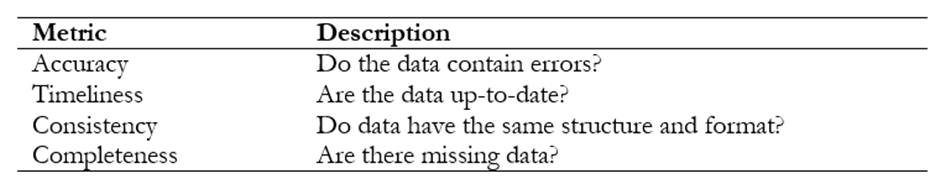
\includegraphics[width=1\textwidth]{SectionIntroduction/introduction_figures/tab_dataQuality.png}
\captionsetup{type=table}
\caption{Metrics to measure the quality of data.}
\label{tab_dataQuality}
\end{figure}

The accuracy identifies if data corresponds to the real values. Timeliness describes if data records are up-to-date (currency) and their update frequency (volatility). Consistency regards the robustness of data format and data structure. Completeness measures the fraction of missing data over the total information content. It is important to check the quality of the input data before starting with data-driven modelling since poor data quality is the most common cause of bad predictions.


%\clearpage
\bibliographystyle{ieeetr}
\bibliography{SectionIntroduction/introduction_ref}



